%%%%%%%%%%%%%%%%%  Debut du fichier Latex  %%%%%%%%%%%%%%%%%%%%%%%%%%%%%%
\documentclass[letterpaper,12pt,onecolumn]{article}

%%% Pour un texte en francais

%%\usepackage[applemac]{inputenc}
%\usepackage[francais]{babel}
	         % encodage des lettres accentuees
\usepackage[T1]{fontenc}
\usepackage[utf8]{inputenc}          % encodage des lettres accentuees
%\usepackage{graphicx}
%%\usepackage{graphicx} \def\BIB{}
\usepackage[paper=a4paper,textwidth=140mm,left=2.1cm,right=2.1cm,top=2.5cm,bottom=2.5cm]{geometry}
\usepackage{multicol}
\usepackage{graphicx,wrapfig,lipsum} 
%\def\BIB{}
\usepackage{caption}
\usepackage{subcaption}
\usepackage[pdftex]{hyperref}
%\usepackage{natbib}
\usepackage{url}
\usepackage{perpage} %the perpage package
\MakePerPage{footnote} %the perpage package command
\hypersetup{
    colorlinks,%
    citecolor=black,%
    filecolor=black,%
    linkcolor=black,%
    urlcolor=blue     % can put red here to visualize the links
}

\usepackage{fancyhdr}
\usepackage{lastpage}

\pagestyle{fancy}
\fancyhf{}
\rhead{Research proposal}
\lhead{El Mellah Ileyk}
\rfoot{\thepage / \pageref{LastPage}}

\DeclareUnicodeCharacter{00A0}{ }

\usepackage{xspace}

%%% Quelques raccourcis pour la mise en page
\newcommand{\remarque}[1]{{\small \it #1}}
\newcommand{\rubrique}{\bigskip \noindent $\bullet$ }
\newcommand{\sgx}{SgXB\xspace}
\newcommand{\ulx}{ULX\xspace}
\newcommand{\sfxt}{SFXT}
\newcommand{\sg}{Sg\xspace}
\newcommand{\co}{CO\xspace}
\newcommand*{\hmxb}{HMXB\@\xspace}
\newcommand*{\lmxb}{LMXB\@\xspace}
\newcommand*{\rlof}{RLOF\@\xspace}
\newcommand*{\ns}{NS\@\xspace}
\newcommand*{\bh}{BH\@\xspace}
\newcommand*{\eg}{e.g.\@\xspace}
\newcommand*{\ie}{i.e.\@\xspace}
\newcommand*{\aka}{a.k.a. \@\xspace}
\newcommand*\diff{\mathop{}\!\mathrm{d}}
\newcommand{\mystar}{{\fontfamily{lmr}\selectfont$\star$}}
\newcommand*{\msun}{$M_{\odot}$\@\xspace}
\newcommand*{\mdotstar}{$\dot{M}_{\text{\mystar}}$\@\xspace}
\newcommand*{\mdotacc}{$\dot{M}_{\text{acc}}$\@\xspace}
\newcommand*{\ledd}{$L_{\text{Edd}}$\@\xspace}


\newcommand{\ignore}[1]{}

\renewcommand*\rmdefault{iwona}

%\pagenumbering{gobble}

%\bibliographystyle{abbrvnat}
%\setcitestyle{authoryear,open={((},close={))}}

%\renewcommand{\thefootnote}{\roman{footnote}}

% -------------------------------------------------
\newcommand{\horrule}[1]{\rule{\linewidth}{#1}} % Create horizontal rule command with 1 argument of height

\title{	
\vspace*{-2.5cm}
%\normalfont \tiny 
%%\textsc{Paris Diderot} \\ [25pt] % Your university, school and/or department name(s)
%\horrule{0.5pt} \\[0.4cm] % Thin top horizontal rule
\Large Speeding up the spinning top\\
\large How accretion sets the pace in High Mass X-ray Binaries  \\ % The assignment title
%\horrule{2pt} \\[0.5cm] % Thick bottom horizontal rule
}
\author{\tiny} % Your name
\date{\tiny }%\normalsize\today} % Today's date or a custom date
% -------------------------------------------------

%\makeatletter
%\def\@xfootnote[#1]{%
%  \protected@xdef\@thefnmark{#1}%
%  \@footnotemark\@footnotetext}
%\makeatother

\usepackage[square,numbers,sort]{natbib}
%\usepackage{har2nat} % "natbib" is loaded automatically

%
%\let\oldthebibliography\thebibliography
%\renewcommand{\thebibliography}[1]{%
%  \oldthebibliography{#1}
%  \let\oldbibitem\bibitem
%  \let\oldtextsc\textsc
%  \def\oldbbland{et}
%  \newcounter{authorcount}
%  \def\bibitem[##1]##2{%
%    \let\textsc\oldtextsc
%    \let\bbland\oldbbland
%    \oldbibitem[##1]{##2}%
%    \let\textsc\mytextsc%
%    \let\bbland\mybbland
%    \setcounter{authorcount}{0}
%  }
%  \def\mybbland{\setcounter{authorcount}{0}\oldbbland}
%  \def\dropetal##1.{ \bbletal}
%  \def\mytextsc##1{%
%    \oldtextsc{##1}%
%    \stepcounter{authorcount}%
%    \ifnum\value{authorcount}=2\relax%
%      \expandafter\dropetal%
%    \fi%
%  }%
%}


\begin{document}

%\bibpunct{[}{]}{;}{n}{,}{,}

%%%%%%%%%%%%%%%%%%%%%%%%%  PREMIERE PAGE %%%%%%%%%%%%%%%%%%%%%%%%%%%%%%
%%% DANS CETTE PAGE, ON REMPLACE LES INDICATIONS ENTRE CROCHETS [...]
%%% PAR LES INFORMATIONS DEMANDEES
%%%%%%%%%%%%%%%%%%%%%%%%%%%%%%%%%%%%%%%%%%%%%%%%%%%%%%%%%%%%%%%%%%%%%%%

%\maketitle
\thispagestyle{empty}

\begin{center}
\Large Speeding up the spinning top\\
\large How accretion sets the pace in High Mass X-ray Binaries 
\end{center}
\normalfont

Massive stars live a forceful life during which they shape galaxies with their mechanical, radiative and chemical feedback. Most of them evolve in a binary system where the two stars orbit close enough from each other to exchange mass, angular momentum and sometimes merge during their evolution \citep{DeMink2012}. Those who remain bounded after the supernova explosion of one the two objects can become a High Mass X-ray Binaries (\hmxb), systems where stellar material is transferred to the compact remnant, either a neutrons star (\ns) or a black hole (\bh). This temporary albeit decisive period in the binary evolution determines its final fate, once a compact binary is formed.

The recent detection of gravitational waves granted us access to the very last moment of this epic journey : the coalescence between two compact objects. It revealed the final masses and effective spins the \bh and \ns involved acquired during their turbulent lifetime \citep{TheLIGOScientificCollaboration2017}. These systems are thought to be the fruit of a massive binary evolution which can lead, under stringent conditions, to compact binaries with orbital separations close enough to spiral-in and merge within a Hubble time.

%\begin{wrapfigure}{o}{0.6\textwidth}
%  \centering
%  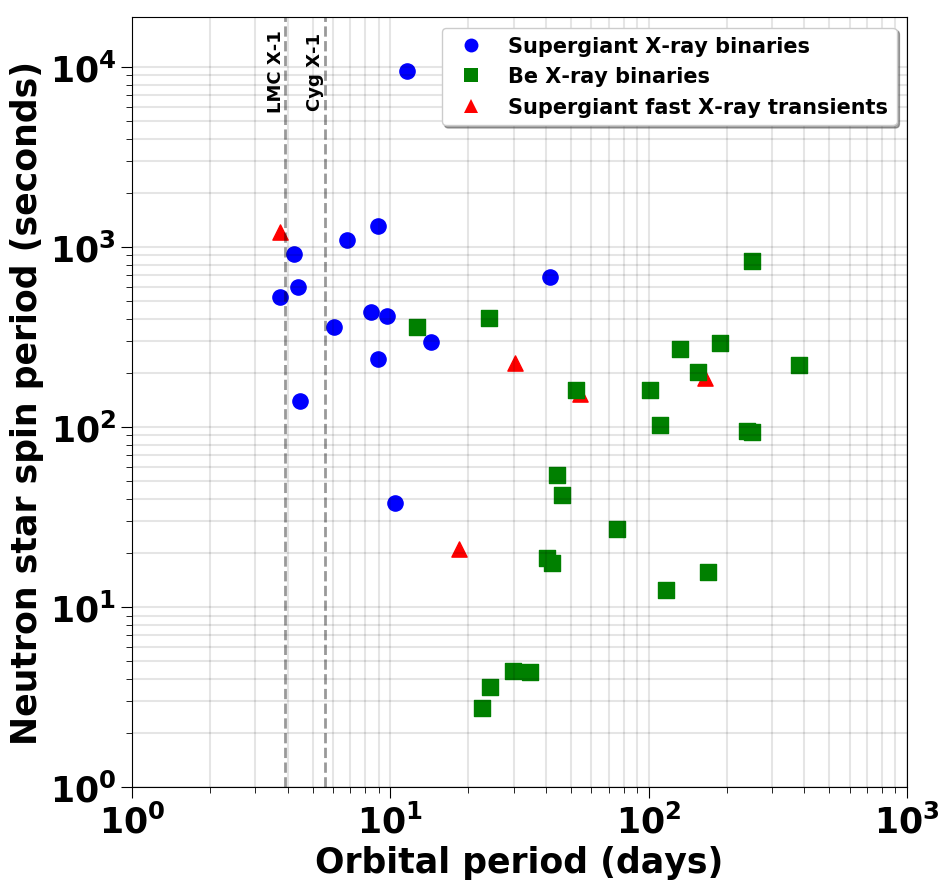
\includegraphics[width=0.6\textwidth]{Figures/corbet_diag.png}
%  \caption{3D contours of the mass density, where the arrows stand for the velocity field in the orbital plane. The central white sphere stands for the inner boundary of the simulation space which represents approximately the outer edge of the \ns magnetosphere, a few 100 times smaller than the outer boundary of the simulation space.}
%  \vspace{-10pt}
%\label{fig:disc}
%\end{wrapfigure}

%\begin{wrapfigure}{o}{0.6\textwidth}
%  \centering
%  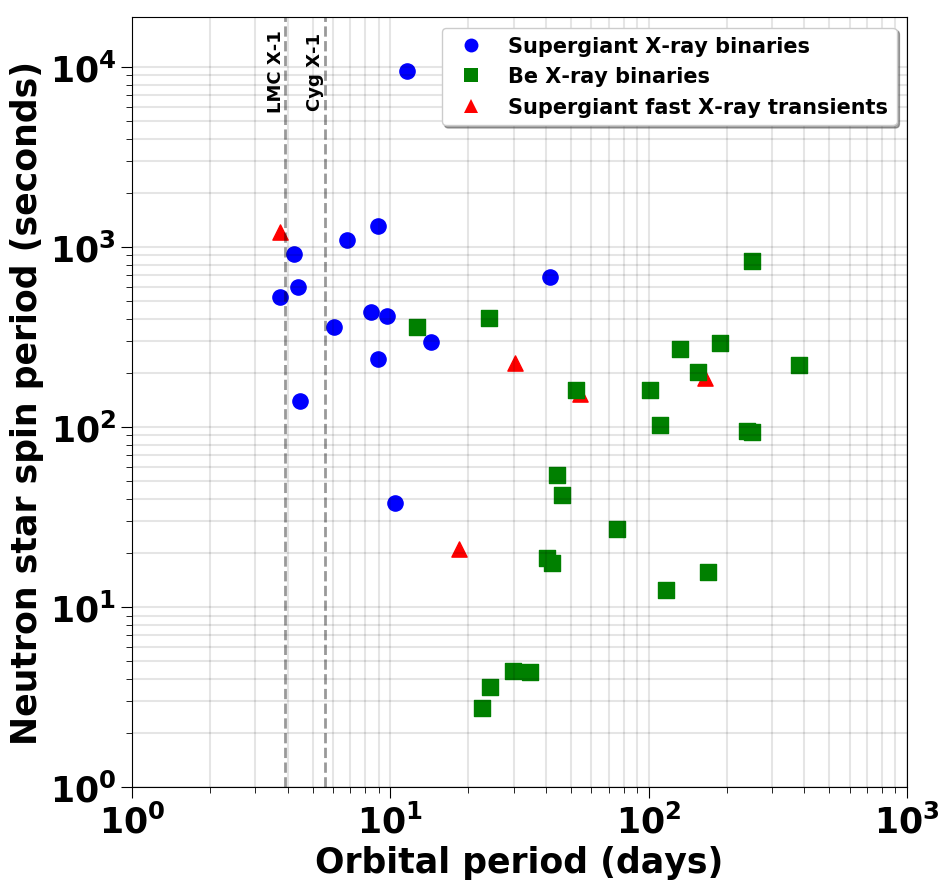
\includegraphics[width=0.6\textwidth]{Figures/corbet_diag.png}
%  \caption{3D contours of the mass density, where the arrows stand for the velocity field in the orbital plane. The central white sphere stands for the inner boundary of the simulation space which represents approximately the outer edge of the \ns magnetosphere, a few 100 times smaller than the outer boundary of the simulation space.}
%  \vspace{-10pt}
%\label{fig:disc}
%\end{wrapfigure}

\begin{figure}[!b]
\centering
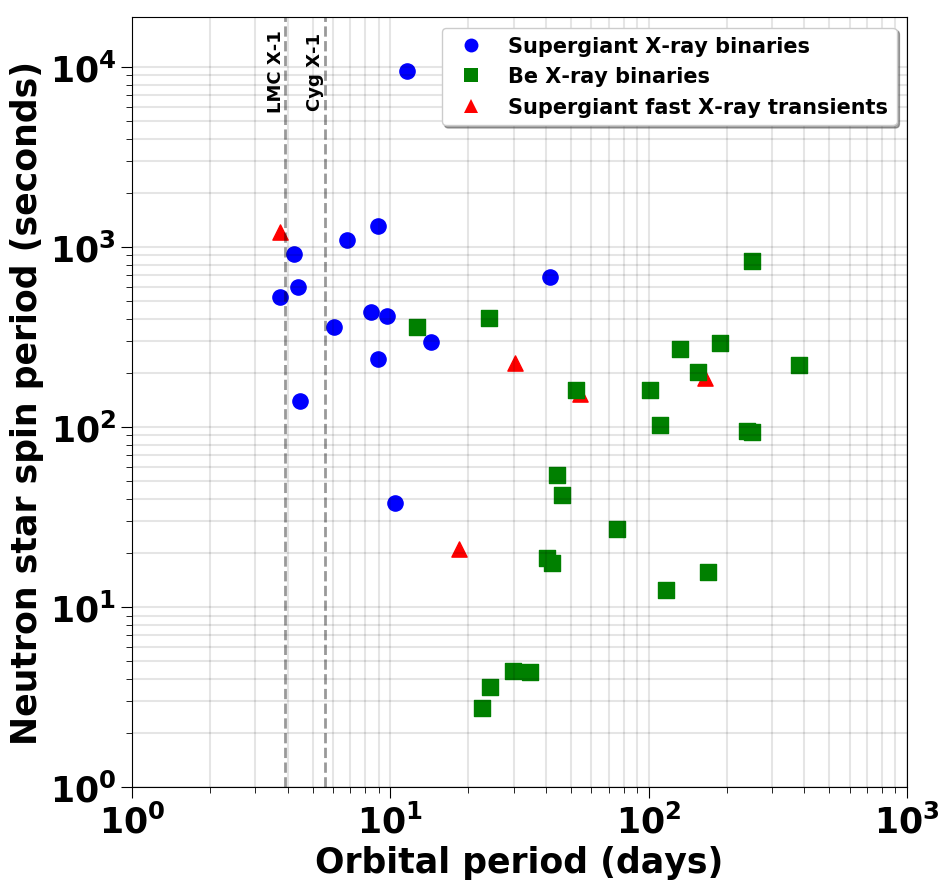
\includegraphics[width=0.6\columnwidth]{Figures/corbet_diag.png}
\caption{Corbet diagram of \ns-hosting Galactic \hmxb with known orbital period. While a correlation exists between the spin and the orbital period in X-ray binaries where the donor star is a massive Be star (a fast rotator surrounded by a decretion disc), it is not the case in \sgx or in Supergiant fast X-ray transients. The orbital periods of the two \bh in \hmxb with measured spins have also been represented (vertical dashed lines).}
\label{fig:spin}
\end{figure} 

Evolutionary models are being developed to predict the upcoming distributions of parameters such as effective spins in \bh-\bh mergers \citep{Belczynski2017} but thorough and repeated observations of individual \hmxb remind us the complexity of phenomena which puts at risk the secular tracks we compute. In particular, the question of the capture of angular momentum by wind-fed compact objects is not settled and need to be addressed to predict the frequency of compact objects mergers and trace back their tumultuous history. For instance, the distribution and secular evolution of the \ns spin in Supergiant X-ray binaries (\sgx, a subclass of \hmxb, see Figure\,\ref{fig:spin}) is the result of intertwined effects : depending on whether the accreted material forms a disc-like structure (prograde or retrograde) before reaching the \ns magnetosphere or remains essentially spherical, the torque applied to the \ns will be significantly different \citep{Ghosh1978,Shakura2012}. However, the spin of the \ns itself can perturb the accretion through magneto-centrifugal effects \citep{Bozzo2008} while the properties of the stellar wind captured determines the geometry of the flow once it reaches the outer rim of the magnetosphere \citep{ElMellah2018}. For accreting \bh, the contribution of ejection via jets or disc winds does not simplify the picture. While some classes of \hmxb show some common angular momentum trends like Be X-ray binaries, others remain out of the scope of our current understanding. The aim of this project is to gather these mechanisms into a consistent frame to address the following core questions :

%The omnipresence of this type of feedback loops in \hmxb between similarly important effects demands to design models where scales are connected and tackle simultaneously the core questions of this project :

%Finally, the X-rays produced as the flow is captured alter the properties of the stellar wind upstream. 

%results of the interaction between the wind of the donor star,  the magnetosphere of the \ns or

%The question of the angular momentum accretion rate onto the compact object is of uttermost importance to 
%is not settled yet.
% far from being solved.

%Dips, off-states, flares, hardening and other short term variability accessible to observational campaigns : our limited understanding of their origin (discs, shocks, jets, large or small scale structures passing by the line-of-sight...) puts at risk the steady picture from which we try to extrapolate the secular evolution.

%In particular, t

%We need to understand how angular momentum was lost and transferred during the \hmxb phase to predict the frequency of compact objects mergers and trace back their tumultuous history. 
%
%To do so, the project will focus on the following core questions :

\begin{enumerate}
\item How does the partial capture of stellar material by the compact object alter the orbital separation and how does it retroactively impact the stellar mass loss?
\item Around a \ns, how does the flow couple to the magnetosphere and what are the short and long term consequences for the spin of the \ns? 
\item For a \bh, how does the spin evolve under the influence of the accretion/ejection trade-off / interplay XXX?
\end{enumerate}

Until now, the several orders of magnitude which separate the orbital scale from the X-ray emitting region, in the immediate vicinity of the compact object, have precluded any bold numerical attempt to follow the accreted flow all along its journey. We were condemned to treat separately the aforementioned problems, presupposing an idealized behavior of the scales out of the scope of the simulation. Within an active collaboration which gathered 20 to 30 observers and theoreticians of winds of massive stars and X-ray binaries over the last years, I have developed and validated a numerical framework which connects these scales and offer the first comprehensive view of mass transfer onto wind-fed compact accretors in binaries. I am now in a position to step forwards and investigate the torques associated, using cutting edge massively parallel codes to solve the radiative magneto-hydrodynamics (RMHD) equations in neatly designed numerical setups. Based on the ample experience I have acquired with these tools, I can reasonably aspire to bring new insights on these questions and contribute to put the newly born field of gravitational wave astronomy into perspective.

%\subsection*{Observational motivations}
%
%If mergers of compact objects set the final state, the simulations I intend to develop feed on observations of the instantaneous state of \hmxb. That is why I have been leading my studies hand in hand with observers, to guarantee the relevance of the numerical setups I designed. The plethora of \hmxb observations carried out thanks to the X-ray instruments in orbit identified the main structures to be modeled in these systems. Orbital-phase resolved spectroscopy performed with the NASA Chandra satellite and the ESA XMM-Newton satellite revealed zones of enhanced ionization and enhanced absorption events \citep{Martinez-Nunez2014,Grinberg2017}. My numerical investigations aim at capturing the dynamics underlying this complex geometry : they disentangle between transient features such as episodic flares due to the micro-structure of the wind \citep{ELMELLAH2017}, and recurring events associated to stable structures present from orbit to orbit such as the bow shock surrounding the accretor \citep{ELMELLAH2015}. The evolution of the spin of the compact object obeys the same logic of systematic and contingent evolution. Although the mass accretion rate might vary little with the geometry of the flow, the long term impact on the torque applied to the compact object can be dramatic. Key simulation parameters are also supplied by the available instruments : in \hmxb hosting a \ns, the observation of cyclotron resonance scattering features with the NASA NuSTAR satellite \citep{Furst2014} sets constrains on the extent of the magnetosphere of direct interest to define representative numerical models of spinning up/down. The wealth of observational data enables us to set a reliable simulation stage to investigate further the coupling between the two spins and the orbital angular momentum via wind accretion and interpret the refined observations of future X-ray satellites.

%INTRODUCE SPIN : MEASURED IN LMXB AND AGN (REF).

\begin{figure}[!b]
\centering
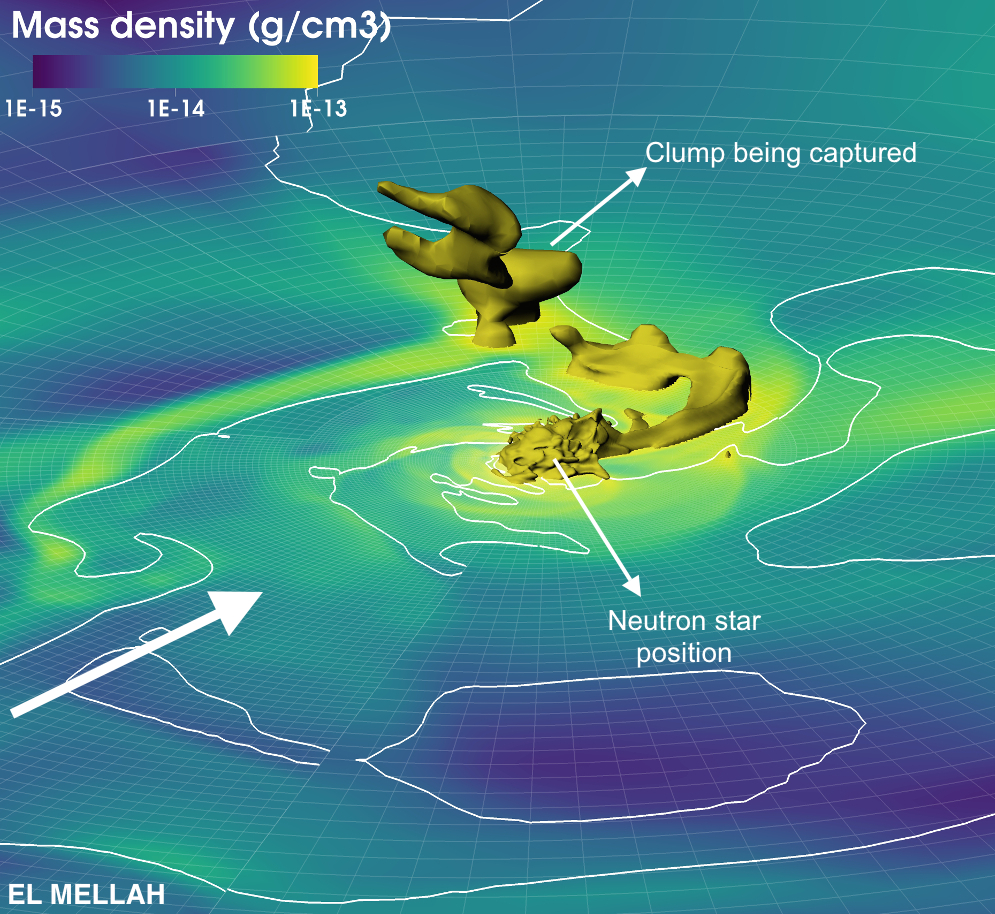
\includegraphics[width=0.65\columnwidth]{Figures/clump_intruder.jpeg}
\caption{Color map slice of the density in the equatorial plane and 3D iso-density surface. The solid white line delimits the Mach-1 surface in the equatorial plane. The accretor lies in the center and the wind comes from the direction bottom left. The capture of an overdense "clump" of matter is visible. The clump carries enough angular momentum to form a transient disc-like structure around the \ns magnetosphere, engulfed in the flow.}
\label{fig:disc}
\end{figure} 

\subsection*{Methodology}

I propose to investigate transfer and loss of angular momentum in \hmxb using RMHD numerical simulations of situations tightly linked to observational signatures. For instance, orbital-phase resolved spectroscopy performed with the NASA Chandra satellite and the ESA XMM-Newton satellite identified the main structures I need to treat in my models of \hmxb (\eg zones of enhanced ionization \citep{Grinberg2017}, accretion tail \citep{Martinez-Nunez2014}...). My numerical investigations aim at capturing the dynamics underlying this complex geometry : they disentangle between stochastic features such as transient discs due to the micro-structure of the wind (see Figure\,\ref{fig:disc} from \cite{ElMellah}), and recurring events associated to stable structures present from orbit to orbit such as the accretion tail in the wake of the accretor \citep{ElMellah2015}.

\begin{itemize}
\item \textbf{\underline{Step 1 : Radiative feedback}} The geometry of the problem (\eg formation of an accretion disc) strongly depends on the capacity of the flow to radiate away its internal energy and compress. Although the mass accretion rate might vary little with the geometry of the flow, the long term impact on the torque applied to the compact object can be dramatic. I implemented a first cooling prescription and used cooling modules suitable for radiatively thin environments, but I now intend to rely on the more realistic treatment of radiative effects available in the \texttt{FLASH} or the \texttt{Athena} codes used by several teams in the US \citep{Jiang2014a}. It will also enable me to extract photometric and spectroscopic synthetic observations from the simulations to be confronted to the observations. For instance, a first publication would assess the possibility for transient truncated discs around \ns to contribute to the soft-excess observed in \ns-\sgx \citep{Bozzo2012}.
\item \textbf{\underline{Step 2 : Coupling with the \ns magnetosphere}} Once the impact of radiative feedback on the geometry is known, we can make use of the multi-scale setup I developed and evaluate, in realistic conditions, the net spinning up or down of a wind-fed \ns. We have semi-analytical expectations for the limit cases, spherical or thin disc geometry, but we can now treat the full 3D time-dependent problem to draw conclusions about the systematic effects which need to be accounted for in computation of population synthesis. A second publication could confront the first synthetic curves of the evolution of the \ns spin as a function of time to the observed ones (\eg in the \ns-hosting Ultra-luminous X-ray source P13, \citep{Fuerst2018}). In specific \sgx like Vela X-1, key simulation parameters such as the extent of the magnetosphere are provided by observations of cyclotron resonance scattering features with the NASA NuSTAR satellite \citep{Furst2014}.
\item \textbf{\underline{Step 3 : The role of outflows}} Stellar winds are an important source of angular momentum loss in \sgx, along with disc winds and jets in some systems like Cygnus X-1 : accretion-ejection in the disc via magneto-centrifugal effects are possible (\eg a Blandford-Payne disc wind) while Blandford-Znajek jets damp the \bh spin in a different way for a prograde or a retrograde disc \citep{Tchekhovskoy2012}. Also, the ejection of stellar material during the common envelope phase can significantly alter the long term evolution of the spins and orbital separation \cite{Murguia-Berthier2017}. If I am granted a Hubble fellowship, the team I would eventually join will influence which aspect I focus more on in this third step. Depending on the skills and centers of interest of the host institution I would be endorsed by, I would set the focus either on the role of outflows in spinning down a wind-fed \bh or on the efficiency of stellar material ejection in the common envelope phase.
\end{itemize}

%I will build up my models hand in hand with 
%
%Step 1 : radiative coupling (ionization of the wind and heating of the inflow => thickness of the disc)
%Step 2 : magnetic component : magnetosphere (produce Pdot diagrams for NS) and turbulent (MRI)
%Step 3 : outflows (MAD, jets...)

\subsection*{Computational tools}


SPINNING UP OF NS ULX REPORTED \citep{Christodoulou2017,Fuerst2018}.

TO SPIN BH, MASSIVE AMOUNT OF MASS REQUIRED


%\section*{Conclusion}
%
%Bedrock model 
%
%Longer term prospective

\newpage

%\newgeometry{left=2cm,right=2cm,top=2.5cm,bottom=2.5cm}
\setlength{\bibsep}{5pt}
\scriptsize
\bibliographystyle{ieeetr}
\bibliography{/Users/Ileyk/Documents/Bibtex/Hubble_fellowship_no_url}

\end{document}
%%%%%%%%%%%%%%%%%  Fin du fichier Latex  %%%%%%%%%%%%%%%%%%%%%%%%%%%%%%

